% !TEX root = ../paper.tex
\subsection{Results of Ease of Use Questionnaire}
Our questionnaire was based on USE, which used Likert scale \ref*{sec:expdesign}, when encoding the data we did it as continuous variable, as such \emph{"strongly disagree"} got a value of 1, and \emph{"strongly agree"} a value ot 7. After that the cumulative value per technique, based on the different questions, was calculated, the data was ploted and presented in \Cref{fig:surveyResult}. 
\begin{figure}[H]
	{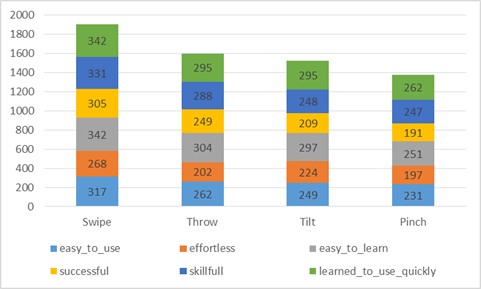
\includegraphics[width = 1\columnwidth , height = 6cm ]{images/survey-data.png}} 
	\caption{
		Cumulative values of survey questions per technique
	}
	\label{fig:surveyResult}
\end{figure}

A One-Way MANOVA was applied ($F(18, 574.66)=5.118,\ p<0.000$) which showed that there is statistical differences between each techniques. 
In order to specify where this differences lie we perform an post hoc test, we summarize the results in regards to each question from the survey, as follow:
\begin{enumerate*}[label=\itshape\arabic*\upshape)]
	\item{``It is easy to use'' \swipe is statistically different, however there is no statistical difference between \throw, \tilt, and \pinch;}
	\item{``Using it is effortless'' \swipe is statistically different, however there is no statistical difference between \throw, \tilt, and \pinch;}
	\item{``It is easy to learn to use''  \swipe and \pinch are statistically different, however there is no statistical difference between \tilt, and \throw;}
	\item{``I can use it successfully every time'' \swipe and \throw are statistically different, there is no statistical difference between \tilt, and \pinch;}
	\item{``I quickly became skillful with it'' \swipe and \throw are statistically different, however there is no statistical difference between \pinch, and \tilt;}
	\item{``I learned how to use it quickly'' \swipe is statistically different, however there is no statistical difference between \throw, \tilt, and \pinch.}
\end{enumerate*}
The results show that the ratings received by the techniques differ in the different aspects of the areas covered by the survey.